\section{Durchführung}
\label{sec:Durchführung}
\subsection{Untersuchung der Filterkurve des Selektivverstärkers}
Zunächst wird die Filterkurve des Selektivverstärkers überprüft. Dafür wird die Ausgangsspannung $U_{\text{A}}$ des Selektivverstärkers bei 
konstanter Eingangsspanung $U_{\text{E}}$  in Abhängigkeit von der Frequenz $\nu$ anhand eines Voltmeters gemessen. Der Frequenzmessbereich befindet sich zwischen
$20$ und $40\,\unit{\kilo\hertz}$, welche mit einem Funktionsgenerator eingestellt werden. Zusätzlich wird die Güte $Q=100$ eingestellt.

\subsection{Messung der Suszeptibilität paramagnetischer Substanzen}
Für die Messung der Suszeptibilität wird der Aufbau aus der Abbildung (\ref{fig:Messapparatur}) verwendet. Zuerst wird die Ausgangsspannung
auf den zuvor bestimmten Maximalwert eingestellt. Dann wird die Brückenschaltung ohne Probe abgeglichen, indem der verstellbarer Widerstand $R_{\text{P}}$
der Brückenschaltung so eingestellt wird, so dass dieser minimal ist. Dazu wird der eingestellte Widerstand und die zugehörige Spannung notiert. Daraufhin 
wird die Probe eingeführt und die Spannung mit der Probe wird gemessen. Daraufhin wird die Brücke mit der Probe erneut abgeglichen. Diese Vorgänge werden jeweils
dreimal für die Proben durchgeführt. Dabei muss beachtet werden, dass die Proben nicht zu lange in der Hand gehalten werden, da der Paramagnetismus stark temperaturabhängig ist.
Da die Proben aus staubförmigen Material bestehen, ist die Dichte der Probe $\rho _{\text{p}}$ geringer als die eines Einkrisstalles $\rho _{\text{w}}$. Demnach gilt für den realen Querschnitt 
\begin{equation}
    Q_{\text{real}}= Q \frac{\rho_{\text{p}}}{\rho_{\text{w}}}\,,
    \label{eqn:Querschnitt}
\end{equation}
mit $Q$ als gemessenen Querschnitt. Außerdem gilt für die Dichte der Probe $\rho_{\text{p}} = \frac{M_{\text{p}}}{Q\, L}$. Hier beschreibt $M_{\text{p}}$  die Masse und
$L$ die Länge der Probe. Daraus folgt
\begin{equation}
    Q_{\text{real}}= \frac{M_{\text{p}}}{L\,\rho_{\text{w}}}\,.
    \label{eqn:Querschnitt_Real}
\end{equation}
Für die in dem Kapitel \ref{sec:Messapparatur_Suszeptibilität}
beschriebenen Messmethoden werden die Messwerte aus der selben Messreihe entnommen. 
\begin{figure}[H]
    \centering
    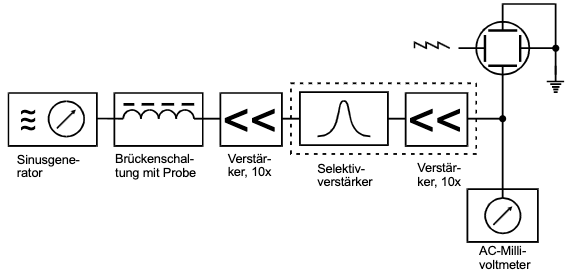
\includegraphics[width = 0.7\textwidth]{content/Bilder/Messapparatur.png}
    \caption{Skizze der Messapparatur zur Bestimmung der Suszeptibilität paramagnetischer Substanzen \cite{anleitungV606}.}
    \label{fig:Messapparatur}
\end{figure} 